\documentclass[11pt]{article}

\usepackage[a4paper,margin=1in]{geometry}
\usepackage{amsmath,amssymb,amsthm}
\usepackage{mathtools}
\usepackage{hyperref}
\usepackage{xcolor}
\usepackage{listings}
\usepackage{booktabs}
\usepackage[T1]{fontenc}
\usepackage{microtype}
\setlength{\emergencystretch}{3em}
\usepackage{tikz}
\usetikzlibrary{arrows.meta,positioning,fit,backgrounds,calc}

% --- Theorem environments ---
\newtheorem{theorem}{Theorem}
\newtheorem{lemma}{Lemma}
\newtheorem{proposition}{Proposition}
\newtheorem{corollary}{Corollary}
\theoremstyle{definition}
\newtheorem{definition}{Definition}
\newtheorem{example}{Example}
\theoremstyle{remark}
\newtheorem{remark}{Remark}

% --- Listings setup for Lean ---
\lstdefinelanguage{Lean}{
  morekeywords={
    import, namespace, end, inductive, def, theorem, abbrev,
    by, intro, apply, exact, simp, constructor, cases, with,
    match, open, have, let, refine, rcases, induction, noncomputable,
    attribute, instance, obtain, by_cases, by_contra, fun, variable,
    termination_by, decreasing_by, return, if, then, else
  },
  sensitive=true,
  morecomment=[l]{--},
  morestring=[b]"
}
\lstset{
  language=Lean,
  basicstyle=\ttfamily\small,
  keywordstyle=\color{blue!60!black},
  commentstyle=\color{green!45!black},
  stringstyle=\color{red!50!black},
  showstringspaces=false,
  breaklines=true,
  frame=single,
  columns=fullflexible,
  mathescape=true,
  literate=
    {á}{{\'{a}}}1
    {é}{{\'{e}}}1
    {í}{{\'{i}}}1
    {ó}{{\'{o}}}1
    {ú}{{\'{u}}}1
    {ñ}{{\~{n}}}1
    {ü}{{\"{u}}}1
    {≤}{{$\leq$}}1
    {≥}{{$\geq$}}1
    {~}{{$\sim$}}1
    {∅}{{$\emptyset$}}1
    {∀}{{$\forall$}}1
    {∃}{{$\exists$}}1
    {→}{{$\to$}}1
    {↔}{{$\leftrightarrow$}}1
    {¬}{{$\neg$}}1
    {∈}{{$\in$}}1
    {∉}{{$\notin$}}1
    {⊆}{{$\subseteq$}}1
    {∧}{{$\land$}}1
    {∨}{{$\lor$}}1
    {≠}{{$\neq$}}1
    {·}{{$\cdot$}}1
    {⟨}{{$\langle$}}1
    {⟩}{{$\rangle$}}1
    {▸}{{$\triangleright$}}1
    {α}{{$\alpha$}}1
    {β}{{$\beta$}}1
    {↑}{{$\uparrow$}}1
    {⊢}{{$\vdash$}}1
    {…}{{$\dots$}}1
    {—}{{---}}1
}

% Pull listings straight from the verified .lean source via marker comments:
% a snippet is delimited by `-- ANCHOR: name` / `-- ANCHOREND: name` and pulled
% with \lstinputlisting[linerange=name-name]{..}; the marker lines are hidden.
\lstset{
  rangebeginprefix=--\ ANCHOR:\ ,
  rangeendprefix=--\ ANCHOREND:\ ,
  includerangemarker=false,
}

% --- Notation in the paper ---
\newcommand{\Perm}{\sim}                         % list permutation
\newcommand{\concat}{\mathbin{+\!\!+}}           % list concatenation ++
\newcommand{\qs}{\operatorname{\mathsf{qsort}}}  % quicksort
\newcommand{\filt}{\operatorname{\mathsf{filter}}}
\newcommand{\len}[1]{\lvert #1 \rvert}
\newcommand{\Sorted}{\operatorname{\mathsf{Ordenada}}}
\DeclareMathOperator{\Pairwise}{Pairwise}

\title{\textbf{Verifying the Correctness of Quicksort in Lean~4}\\[2pt]
\large A machine-checked proof that quicksort returns a sorted permutation}
\author{\textbf{Rudik Rompich} \\ Universidad del Valle de Guatemala \\ \texttt{rom19857@uvg.edu.gt}}
\date{June 2026}

\begin{document}
\maketitle

\begin{abstract}
This report gives a complete, machine-checked proof that the classical functional
\emph{quicksort} algorithm is correct: on any input list over a linearly ordered type, it
returns a list that is (i)~\emph{sorted} in nondecreasing order and (ii)~a~\emph{permutation}
of the input. We first explain what the algorithm is and what ``correct'' precisely means,
illustrate the divide-and-conquer structure with diagrams, and develop the full mathematical
argument---termination, the permutation property, and the sortedness property---at the level
of detail expected in a rigorous proof. Each mathematical step is then mirrored by its Lean~4
realization, so that the reader can see that the Lean terms genuinely prove the stated theorems.
The development uses no \texttt{sorry} and no postulated lemma; an axiom audit confirms that the
final theorem depends on \texttt{propext} and \texttt{Quot.sound}, without \texttt{Classical.choice}.
\end{abstract}

\tableofcontents

\section{What the problem is}
\label{sec:problem}

\subsection{Sorting and its specification}
A \emph{sorting algorithm} takes a finite sequence of elements drawn from a totally ordered
domain and rearranges them into nondecreasing order. ``Rearranges'' is the crucial word: a
sorting algorithm is not allowed to invent, drop, or duplicate elements. Hence correctness has
\emph{two} independent parts, and both are needed:

\begin{enumerate}
\item \textbf{Sortedness.} The output is in nondecreasing order.
\item \textbf{Permutation.} The output contains exactly the same elements as the input, with the
same multiplicities (it is a rearrangement).
\end{enumerate}

Neither half suffices alone. The constant function returning \texttt{[]} produces a sorted list
but is not a permutation; the identity function is a permutation but not sorted. Only their
conjunction pins down ``sorting''. We therefore adopt the following specification.

\begin{definition}[Sorting function]\label{def:spec}
Let $(\alpha,\leq)$ be a linearly ordered type. A function $f:\mathrm{List}\,\alpha\to
\mathrm{List}\,\alpha$ \emph{sorts} if for every list $\ell$,
\[
  f(\ell)\ \Perm\ \ell
  \qquad\text{and}\qquad
  \Sorted\big(f(\ell)\big),
\]
where $\Perm$ denotes ``is a permutation of'' and $\Sorted$ denotes ``is in nondecreasing
order''. Our goal is to prove that quicksort satisfies both conjuncts.
\end{definition}

\subsection{What ``sorted'' means, precisely}
We take the order-theoretic definition that is easiest to reason about inductively: a list is
sorted when \emph{every element precedes (or equals) every later element}.

\begin{definition}[Ordenada]\label{def:sorted}
A list $\ell=[a_0,a_1,\dots,a_{n-1}]$ is \emph{sorted} if $a_i\leq a_j$ whenever $i\leq j$.
Equivalently, writing the predicate as a pairwise relation,
\[
  \Sorted(\ell)\ \ :\Longleftrightarrow\ \ \Pairwise\,(\leq)\,\ell,
\]
i.e.\ for every way of choosing an earlier element $a$ and a later element $b$ in $\ell$, we have
$a\leq b$.
\end{definition}

The pairwise formulation is convenient because it splits cleanly over concatenation, which is
exactly the operation quicksort uses to assemble its output (Lemma~\ref{lem:pairwise-append}).

\subsection{What ``permutation'' means, precisely}
\begin{definition}[Permutation]\label{def:perm}
Two lists are \emph{permutations} of each other, written $\ell_1\Perm\ell_2$, if one can be
obtained from the other by reordering. Formally, $\Perm$ is the smallest equivalence relation on
lists closed under swapping adjacent elements; equivalently, $\ell_1\Perm\ell_2$ iff every value
occurs the same number of times in $\ell_1$ as in $\ell_2$. Permutation is reflexive, symmetric
and transitive, is a congruence for concatenation ($\ell_1\Perm\ell_1'$ and $\ell_2\Perm\ell_2'$
imply $\ell_1\concat\ell_2\Perm\ell_1'\concat\ell_2'$), and implies equality of membership
($a\in\ell_1\leftrightarrow a\in\ell_2$).
\end{definition}

These standard closure properties of $\Perm$ are the only facts about permutations we will use;
in Lean they are \texttt{Perm.append}, \texttt{Perm.cons}, \texttt{Perm.trans}, \texttt{perm\_middle},
and \texttt{Perm.mem\_iff}.

\section{The algorithm}
\label{sec:algorithm}

Quicksort (C.~A.~R.~Hoare, 1961) is a \emph{divide-and-conquer} algorithm. Given a nonempty
list, it chooses one element as the \emph{pivot}\,---we take the head\,---and partitions the
remaining elements into those that are $\leq$ the pivot and those that are $>$ the pivot. Each
part is sorted recursively, and the sorted parts are concatenated with the pivot placed in
between. The empty list is already sorted.

\begin{definition}[Functional quicksort]\label{def:qs}
Over a linearly ordered type $\alpha$, define $\qs:\mathrm{List}\,\alpha\to\mathrm{List}\,\alpha$
by
\[
  \qs([]) = [], \qquad
  \qs(p :: r) = \qs(\ell_{\leq})\ \concat\ \big(p :: \qs(\ell_{>})\big),
\]
where, from the tail $r$, the two partition halves are
\[
  \ell_{\leq} \;=\; \filt(\lambda x.\,x\leq p)\,(r),
  \qquad
  \ell_{>} \;=\; \filt(\lambda x.\,\neg(x\leq p))\,(r).
\]
Here $p$ is the pivot, $::$ is ``cons'' (prepend), and $\concat$ is concatenation. Note
$\ell_{>}$ collects exactly the elements failing the test $x\leq p$, i.e.\ those with $p<x$.
\end{definition}

\subsection{Picture: one level of divide-and-conquer}
A single recursive step rearranges the input around the pivot as follows. The key structural
fact---which drives the sortedness proof---is that \emph{everything to the left of the pivot is
$\leq p$ and everything to its right is $>p$}.

\begin{center}
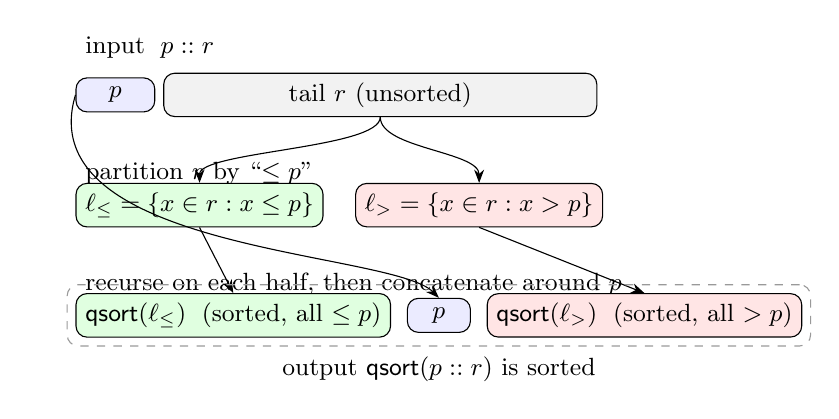
\begin{tikzpicture}[font=\small,node distance=2mm]
  % input
  \node (inlabel) {input \;$p :: r$};
  \node[draw, rounded corners, fill=blue!8, minimum width=1cm, below=6mm of inlabel.west, anchor=west] (p0) {$p$};
  \node[draw, rounded corners, fill=gray!10, minimum width=5.5cm, right=1mm of p0] (r0) {tail $r$ (unsorted)};

  % partition
  \node[below=10mm of p0.west, anchor=west] (partlabel) {partition $r$ by ``$\leq p$''};
  \node[draw, rounded corners, fill=green!12, minimum width=3cm, below=4mm of partlabel.west, anchor=west] (le) {$\ell_{\leq}=\{x\in r: x\leq p\}$};
  \node[draw, rounded corners, fill=red!10, minimum width=3cm, right=4mm of le] (gt) {$\ell_{>}=\{x\in r: x> p\}$};

  % recurse + combine
  \node[below=10mm of le.west, anchor=west] (comblabel) {recurse on each half, then concatenate around $p$};
  \node[draw, rounded corners, fill=green!12, minimum width=3cm, below=4mm of comblabel.west, anchor=west] (qle) {$\qs(\ell_{\leq})$ \;(sorted, all $\leq p$)};
  \node[draw, rounded corners, fill=blue!8, minimum width=0.8cm, right=2mm of qle] (pp) {$p$};
  \node[draw, rounded corners, fill=red!10, minimum width=3cm, right=2mm of pp] (qgt) {$\qs(\ell_{>})$ \;(sorted, all $> p$)};

  \draw[-{Stealth}] (r0.south) .. controls +(0,-0.4) and +(0,0.4) .. (le.north);
  \draw[-{Stealth}] (r0.south) .. controls +(0,-0.4) and +(0,0.4) .. (gt.north);
  \draw[-{Stealth}] (le.south) -- (qle.north);
  \draw[-{Stealth}] (gt.south) -- (qgt.north);
  \draw[-{Stealth}] (p0.west) .. controls +(-0.6,-2) and +(-0.6,0.6) .. (pp.north);

  \node[draw=black!40, dashed, rounded corners, fit=(qle)(pp)(qgt), inner sep=3pt, label=below:{output $\qs(p::r)$ is sorted}] {};
\end{tikzpicture}
\end{center}

\subsection{Picture: the recursion tree}
Unfolding the recursion on a concrete input produces a binary tree. Each node is labeled by its
pivot (the head); its left child handles the elements $\leq$ the pivot, its right child the
elements $>$ the pivot. Reading the leaves and pivots in in-order (left subtree, pivot, right
subtree) yields the sorted output.

\begin{center}
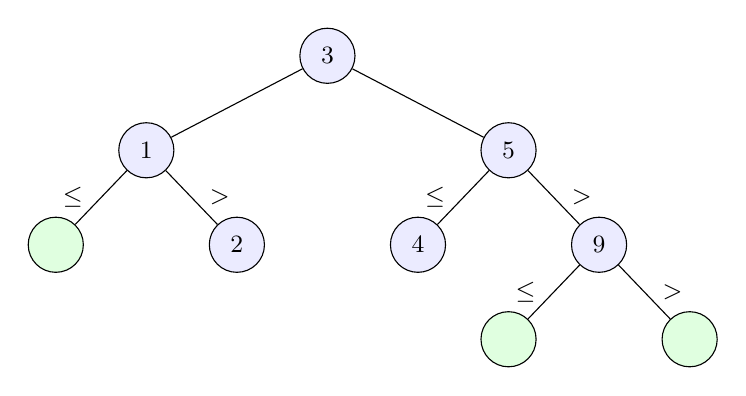
\begin{tikzpicture}[font=\small,level distance=12mm,
  level 1/.style={sibling distance=46mm},
  level 2/.style={sibling distance=23mm},
  every node/.style={draw,circle,inner sep=1.4pt,minimum size=7mm,fill=blue!8}]
  \node {3}
    child { node {1}
      child { node[fill=green!12] {} edge from parent node[draw=none,fill=none,left]{$\leq$} }
      child { node {2} edge from parent node[draw=none,fill=none,right]{$>$} }
    }
    child { node {5}
      child { node {4} edge from parent node[draw=none,fill=none,left]{$\leq$} }
      child { node {9}
        child { node[fill=green!12] {} edge from parent node[draw=none,fill=none,left]{$\leq$}}
        child { node[fill=green!12] {} edge from parent node[draw=none,fill=none,right]{$>$}}
        edge from parent node[draw=none,fill=none,right]{$>$} }
    };
\end{tikzpicture}
\end{center}

\noindent For the input $[3,1,2,5,4,9]$ the root pivot is $3$; the left half $[1,2]$ (elements
$\leq3$) recurses with pivot $1$, the right half $[5,4,9]$ (elements $>3$) recurses with pivot
$5$, and so on. Empty leaves (shaded) are the base case $\qs([])=[]$. In-order traversal gives
$1,2,3,4,5,9$.

\subsection{Lean: the definition}
The Lean text below is the literal definition. The Boolean test \texttt{decide (x $\leq$ p)} turns
the decidable proposition $x\leq p$ into a \texttt{Bool} so that it can drive \texttt{List.filter};
its negation \texttt{!\,decide (x $\leq$ p)} selects the complementary half.

\lstinputlisting[linerange=filterDecrease-filterDecrease]{../../Thesis/Sort/Quicksort.lean}
\lstinputlisting[linerange=qsdef-qsdef]{../../Thesis/Sort/Quicksort.lean}

\section{Termination}
\label{sec:termination}

Quicksort does not recurse on a structural subterm (the halves are \emph{computed} by filtering,
not pattern-matched), so before we can even speak of $\qs$ as a total function we must prove that
the recursion terminates. The measure is the \emph{length} of the argument.

\begin{lemma}[Filtering does not increase length]\label{lem:filter-le}
For any predicate $q$ and list $\ell$, $\ \len{\filt(q)(\ell)}\leq\len{\ell}$.
\end{lemma}
\begin{proof}
Induction on $\ell$. For $\ell=[]$ both sides are $0$. For $\ell=a::\ell'$, filtering either keeps
$a$ (length $1+\len{\filt(q)(\ell')}$) or drops it (length $\len{\filt(q)(\ell')}$); in both cases
the result is $\leq 1+\len{\ell'}=\len{\ell}$ using the induction hypothesis.
\end{proof}

\begin{proposition}[Termination]\label{prop:term}
Each recursive call of $\qs(p::r)$ is on a strictly shorter list, so $\qs$ is a total function.
\end{proposition}
\begin{proof}
The recursive arguments are $\ell_{\leq}=\filt(\cdot\leq p)(r)$ and $\ell_{>}=\filt(\neg(\cdot\leq
p))(r)$. By Lemma~\ref{lem:filter-le}, $\len{\ell_{\leq}}\leq\len{r}$ and
$\len{\ell_{>}}\leq\len{r}$. Since $\len{p::r}=\len{r}+1>\len{r}$, both recursive arguments are
strictly shorter than the input. Well-founded recursion on $\len{\cdot}$ (a $\mathbb{N}$-valued
measure) is therefore justified.
\end{proof}

\subsection{Lean: discharging the termination obligations}
After \texttt{termination\_by l => l.length}, each recursive argument must be shorter than
the input. The helper \texttt{longitud\_filtro\_lt\_cons} combines the two bounds
\[
  \len{\filt(q)(r)}\ \leq\ \len{r}<\len{p::r}.
\]
The first is \texttt{length\_filter\_le} (Lemma~\ref{lem:filter-le}); the second is
\texttt{Nat.lt\_succ\_self}. In the definition of the algorithm,
\texttt{unattach\_filter} and \texttt{unattach\_attach} remove Lean's internal membership
annotations before this helper is applied to each partition predicate.

\noindent Because the definition uses well-founded (not structural) recursion, the equation
$\qs([])=[]$ and the unfolding for $p::r$ are not definitional; Lean provides them as rewrite
lemmas, which we name for use in proofs:

\lstinputlisting[linerange=qsequations-qsequations]{../../Thesis/Sort/Quicksort.lean}

\section{The specification in Lean}
\label{sec:spec-lean}

We render Definition~\ref{def:sorted} directly: ``sorted'' is the pairwise-$\leq$ predicate.

\lstinputlisting[linerange=sortedDef-sortedDef]{../../Thesis/Sort/Quicksort.lean}

\noindent The two conjuncts of Definition~\ref{def:spec} become \texttt{quicksort l \~{} l} (the
permutation, using Lean's notation \texttt{\~{}} for \texttt{List.Perm}) and \texttt{Ordenada
(quicksort l)}. We prove them separately (\S\ref{sec:perm} and \S\ref{sec:sorted}) and then
combine them (\S\ref{sec:correct}).

\section{Correctness, part I: the output is a permutation}
\label{sec:perm}

\subsection{Mathematics}
We first record the one combinatorial fact about filtering that the proof needs: splitting a list
by a Boolean test and concatenating the two halves is a permutation of the original.

\begin{lemma}[Filter partition is a permutation]\label{lem:filter-perm}
For any Boolean test $q$ and list $\ell$,
\[
  \filt(q)(\ell)\ \concat\ \filt(\lambda x.\,\neg q\,x)(\ell)\ \ \Perm\ \ \ell .
\]
\end{lemma}
\begin{proof}
Induction on $\ell$. The empty case is reflexivity. For $\ell=a::\ell'$, distinguish whether $a$
passes the test. If $q\,a$ holds, the left half is $a::\filt(q)(\ell')$ and the right half is
$\filt(\lambda x.\,\neg q\,x)(\ell')$, so the concatenation is $a::\big(\filt(q)(\ell')\concat
\filt(\lambda x.\,\neg q\,x)(\ell')\big)$, which by the induction hypothesis is $\Perm\,a::\ell'$.
If $q\,a$ fails, the element $a$ is the head of the \emph{right} half; the concatenation is
$\filt(q)(\ell')\concat\big(a::\filt(\lambda x.\,\neg q\,x)(\ell')\big)$, and moving $a$ to the
front (a permutation, since adjacent transpositions generate $\Perm$) reduces again to the
induction hypothesis.
\end{proof}

\begin{theorem}[Permutation]\label{thm:perm}
For every list $\ell$, $\ \qs(\ell)\Perm\ell$.
\end{theorem}
\begin{proof}
By well-founded induction on $\len{\ell}$ (legitimate by Proposition~\ref{prop:term}). If
$\ell=[]$, then $\qs([])=[]\Perm[]$. If $\ell=p::r$, the two recursive calls are on the shorter
lists $\ell_{\leq}$ and $\ell_{>}$, so the induction hypothesis gives
\[
  \qs(\ell_{\leq})\Perm\ell_{\leq}
  \qquad\text{and}\qquad
  \qs(\ell_{>})\Perm\ell_{>}.
\]
Using that $\Perm$ is a congruence for $\concat$ and for $::$,
\[
  \underbrace{\qs(\ell_{\leq})\concat\big(p::\qs(\ell_{>})\big)}_{=\,\qs(p::r)}
  \ \Perm\
  \ell_{\leq}\concat\big(p::\ell_{>}\big).
\]
Next, pull the pivot to the front---$\ell_{\leq}\concat(p::\ell_{>})\Perm
p::(\ell_{\leq}\concat\ell_{>})$, an instance of the ``middle'' permutation---and finally apply
Lemma~\ref{lem:filter-perm} under the head $p$:
\[
  p::(\ell_{\leq}\concat\ell_{>})\ \Perm\ p::r .
\]
Chaining these by transitivity yields $\qs(p::r)\Perm p::r$.
\end{proof}

\begin{corollary}[Membership is preserved]\label{cor:mem}
For all $a$ and $\ell$, $\ a\in\qs(\ell)\leftrightarrow a\in\ell$.
\end{corollary}
\begin{proof}
Immediate from Theorem~\ref{thm:perm}, since permutations have the same members.
\end{proof}

\subsection{Lean}
The hypotheses \texttt{hipIndMenoresIguales} and \texttt{hipIndMayores} are recursive calls on the shorter
partitions. The named steps \texttt{hDerecha}, \texttt{hConcatenacion}, \texttt{hPivote}, and
\texttt{hParticion} expose the congruence and partition arguments; the final
\texttt{calc} displays the intermediate lists explicitly.

\lstinputlisting[linerange=perm-perm]{../../Thesis/Sort/Quicksort.lean}

\section{Correctness, part II: the output is sorted}
\label{sec:sorted}

\subsection{Mathematics}
The sortedness proof rests on how the pairwise predicate behaves under concatenation, and on the
defining property of the two partition halves.

\begin{lemma}[Pairwise over concatenation]\label{lem:pairwise-append}
For a relation $R$ and lists $\ell_1,\ell_2$,
\[
  \Pairwise\,R\,(\ell_1\concat\ell_2)
  \ \Longleftrightarrow\
  \Pairwise\,R\,\ell_1 \ \wedge\ \Pairwise\,R\,\ell_2 \ \wedge\
  \big(\forall a\in\ell_1,\ \forall b\in\ell_2,\ R\,a\,b\big).
\]
Likewise $\Pairwise\,R\,(a::\ell)\Leftrightarrow(\forall b\in\ell,\ R\,a\,b)\wedge\Pairwise\,R\,\ell$.
\end{lemma}
\begin{proof}
Standard, by induction on $\ell_1$ (resp.\ unfolding the cons case). These are library facts
(\texttt{List.pairwise\_append}, \texttt{List.pairwise\_cons}).
\end{proof}

The decisive observation is the \emph{separation} guaranteed by the partition: every element of
the menoresIguales half is $\leq p$ and every element of the mayores half is $>p$ (hence $\geq p$). Combined
with transitivity of $\leq$, this gives the cross-bound needed to glue the recursively sorted
halves.

\begin{theorem}[Sortedness]\label{thm:sorted}
For every list $\ell$, $\ \Sorted(\qs(\ell))$.
\end{theorem}
\begin{proof}
By well-founded induction on $\len{\ell}$. The empty list is vacuously sorted. Let $\ell=p::r$,
and abbreviate $A=\qs(\ell_{\leq})$ and $B=\qs(\ell_{>})$, so $\qs(\ell)=A\concat(p::B)$. The
induction hypothesis gives $\Sorted(A)$ and $\Sorted(B)$.

\emph{Bounds on the halves.} Let $a\in A$. By Corollary~\ref{cor:mem}, $a\in\ell_{\leq}$, i.e.\ $a$
occurs in $r$ and passes the test, so $a\leq p$. Let $b\in B$. Again by
Corollary~\ref{cor:mem}, $b\in\ell_{>}$, i.e.\ $b$ occurs in $r$ and fails the test $b\leq p$;
since $\leq$ is a linear order, $\neg(b\leq p)$ gives $p<b$, hence $p\leq b$. Summarizing:
\[
  (\forall a\in A,\ a\leq p)
  \qquad\text{and}\qquad
  (\forall b\in B,\ p\leq b). \tag{$\ast$}
\]

\emph{Assembling.} By Lemma~\ref{lem:pairwise-append} applied to $A\concat(p::B)$, sortedness of
the whole reduces to three obligations:
\begin{enumerate}
\item $\Sorted(A)$: the induction hypothesis.
\item $\Sorted(p::B)$: by the cons-form of Lemma~\ref{lem:pairwise-append}, this needs
$(\forall b\in B,\ p\leq b)$---the right half of $(\ast)$---together with $\Sorted(B)$, the
induction hypothesis.
\item Cross-bound: $\forall a\in A,\ \forall c\in (p::B),\ a\leq c$. Fix $a\in A$ and
$c\in p::B$. If $c=p$, then $a\leq p$ by the left half of $(\ast)$. If $c\in B$, then
$a\leq p\leq c$ by both halves of $(\ast)$ and transitivity of $\leq$.
\end{enumerate}
All three hold, so $\Sorted(A\concat(p::B))=\Sorted(\qs(\ell))$.
\end{proof}

\subsection{Picture: why the assembled list is sorted}
The three obligations above correspond exactly to the three ``zones'' of the output and the
order relations between them:

\begin{center}
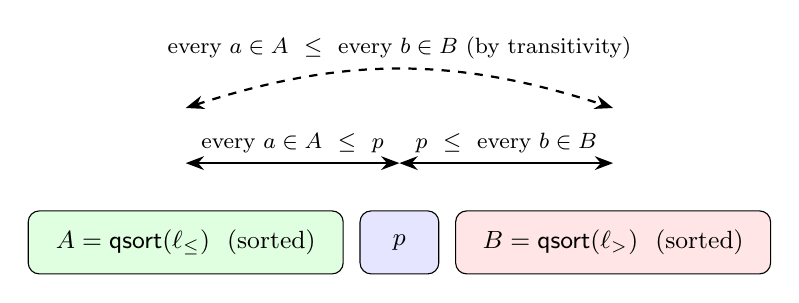
\begin{tikzpicture}[font=\small]
  \node[draw, rounded corners, fill=green!12, minimum width=4cm, minimum height=8mm] (A) {$A=\qs(\ell_{\leq})$ \ (sorted)};
  \node[draw, rounded corners, fill=blue!10, minimum width=1cm, minimum height=8mm, right=2mm of A] (p) {$p$};
  \node[draw, rounded corners, fill=red!10, minimum width=4cm, minimum height=8mm, right=2mm of p] (B) {$B=\qs(\ell_{>})$ \ (sorted)};

  \draw[{Stealth}-{Stealth}, thick] ([yshift=6mm]A.north) -- node[above]{\footnotesize every $a\in A$ \ $\leq$ \ $p$} ([yshift=6mm]p.north);
  \draw[{Stealth}-{Stealth}, thick] ([yshift=6mm]p.north) -- node[above]{\footnotesize $p$ \ $\leq$ \ every $b\in B$} ([yshift=6mm]B.north);
  \draw[{Stealth}-{Stealth}, thick, dashed] ([yshift=13mm]A.north) to[bend left=18] node[above]{\footnotesize every $a\in A$ \ $\leq$ \ every $b\in B$ (by transitivity)} ([yshift=13mm]B.north);
\end{tikzpicture}
\end{center}

\noindent Within $A$ and within $B$ order holds by the induction hypothesis; across the pivot it
holds by the partition bounds $(\ast)$; and the long-range bound $A$-to-$B$ follows by chaining
through $p$. These are precisely obligations (1)--(3).

\subsection{Lean}
The Lean proof names the same pieces: \texttt{hipIndMenoresIguales}, \texttt{hipIndMayores} are $\Sorted(A)$, $\Sorted(B)$;
\texttt{hCotaMenoresIguales}, \texttt{hCotaMayores} are the two halves of $(\ast)$, each obtained by transporting
membership back through \texttt{pertenencia\_quicksort} (Corollary~\ref{cor:mem}) and unfolding the filter
test; \texttt{pairwise\_append} and \texttt{pairwise\_cons} are Lemma~\ref{lem:pairwise-append};
and the final \texttt{le\_trans} is the transitivity step of obligation~(3).

\lstinputlisting[linerange=sorted_thm-sorted_thm]{../../Thesis/Sort/Quicksort.lean}

\section{Correctness}
\label{sec:correct}

Putting the two halves together gives the specification of Definition~\ref{def:spec}.

\begin{theorem}[Correctness of quicksort]\label{thm:correct}
For every list $\ell$ over a linearly ordered type,
\[
  \qs(\ell)\Perm\ell \quad\text{and}\quad \Sorted(\qs(\ell)).
\]
That is, quicksort returns a sorted permutation of its input.
\end{theorem}
\begin{proof}
The first conjunct is Theorem~\ref{thm:perm}; the second is Theorem~\ref{thm:sorted}.
\end{proof}

\lstinputlisting[linerange=correct-correct]{../../Thesis/Sort/Quicksort.lean}

\section{Worked examples}
\label{sec:examples}

Because $\qs$ is an ordinary computable function, we can both \emph{run} it and \emph{prove}
facts about concrete inputs by specializing the general theorems---no recomputation or
\texttt{decide} is required.

\lstinputlisting[linerange=examples-examples]{../../Thesis/Sort/Examples.lean}

\noindent The example \texttt{[2, 1, 2, 1]\,$\mapsto$\,[1, 1, 2, 2]} illustrates that quicksort is a
\emph{permutation}, not a deduplication: both copies of each value survive, which is exactly what
Theorem~\ref{thm:perm} guarantees.

\section{Verification: the axiom audit}
\label{sec:axioms}

A formal proof is only as trustworthy as its hidden assumptions. Two failure modes must be
excluded: an admitted gap (\texttt{sorry}, which surfaces as the pseudo-axiom \texttt{sorryAx})
and a silently postulated lemma. Lean's \texttt{\#print axioms} reports the complete transitive
axiom dependency of a theorem. Running it on the main result yields:

% Generated by `make audit-quicksort` from Thesis/Sort/Audit.lean — do not edit by hand.
\lstinputlisting[language={},basicstyle=\ttfamily\footnotesize]{audit.txt}

\noindent The reported axioms are \texttt{propext} (propositional extensionality) and
\texttt{Quot.sound} (correccion of quotients). The explicit termination proof no longer
introduces a dependency on \texttt{Classical.choice}. This reports the dependencies of these
terms, not a minimal foundation for the theorem. Crucially, \texttt{sorryAx} does \emph{not} appear: there are no admitted gaps, and
no postulated sorting or correctness lemma is used. This is the formal certificate that
Theorem~\ref{thm:correct} is exactly what it claims to be.

\section{Cross-validation by an automated prover (Harmonic Aristotle)}
\label{sec:aristotle}
As an independent check on the result, we asked Harmonic's automated theorem prover
\emph{Aristotle}~\cite{Aristotle} to reconstruct the correctness proof \emph{cold}. Aristotle works
inside Lean~4 and discharges every goal through the same kernel used here, so whatever it produces is
verified to the identical standard---it is not an oracle, but a proof-search procedure whose output is
a checkable Lean term.

\paragraph{Protocol.} Aristotle was given only the definition of \texttt{Ordenada}, the recursive
definition of \texttt{quicksort}, and its unfolding equation \texttt{quicksort\_cons}; the correctness
theorem was presented as a bare \texttt{sorry}, and the permutation and sortedness lemmas were
\emph{withheld}. It was instructed to complete the proof introducing no axioms and no \texttt{sorry}.
Every artifact below compiles under the same Lean~v4.29.0 toolchain as the cola of this development and
passes the axiom audit of \S\ref{sec:axioms}.

\paragraph{Result.} Aristotle rediscovered the same two-lemma decomposition---establish a permutation
lemma and a sortedness lemma, then conjoin them---under the same names. Its \emph{sortedness} proof
follows essentially our argument (\texttt{pairwise\_append}/\texttt{pairwise\_cons} together with the
pivot's separation bounds). For \emph{permutation}, however, it took a genuinely different route: where
our proof rearranges the partitions structurally (Lemma~\ref{lem:filter-perm} and \texttt{perm\_middle}),
Aristotle reduced $\Perm$ to equality of element \emph{multiplicities} (\texttt{List.perm\_iff\_count})
and closed the resulting counting goal by automation:

\lstinputlisting[linerange=qaperm-qaperm]{../../aristotle/QuicksortFull.lean}

\noindent It then assembled correctness exactly as we do:

\lstinputlisting[linerange=qamain-qamain]{../../aristotle/QuicksortFull.lean}

\paragraph{What differs, and what does not.} Mathematically the two developments agree: correctness is
\emph{permutation $\wedge$ sortedness}, each proved by induction on length. They differ in idiom---the
hand proof is structured and explicit, while Aristotle leans on Mathlib's general-purpose automation
(\texttt{grind}, \texttt{aesop}, \texttt{simp\,+decide}) and on a counting characterization of
permutation. The Aristotle reconstruction retains its original audit dependencies
\texttt{[propext, Classical.choice, Quot.sound]}; the revised local proof reports only
\texttt{[propext, Quot.sound]}. Both avoid \texttt{sorryAx}, but their dependency lists
are not identical.

\section{Conclusion}
\label{sec:conclusion}

We have given a complete, kernel-checked proof that functional quicksort meets the specification
of a sorting algorithm:
\[
  \qs(\ell)\Perm\ell \quad\text{and}\quad \Sorted(\qs(\ell)) \qquad\text{for every list }\ell.
\]
The argument has three mathematically distinct ingredients, each mirrored exactly in Lean:
\emph{termination} by the length measure (Proposition~\ref{prop:term}), the \emph{permutation}
property via the filter-partition lemma and the congruence/middle properties of $\Perm$
(Theorem~\ref{thm:perm}), and the \emph{sortedness} property via the partition's separation
bounds, the behaviour of \texttt{Pairwise} under concatenation, and transitivity of the order
(Theorem~\ref{thm:sorted}). The axiom audit (\S\ref{sec:axioms}) certifies the proof is free of
admitted gaps and of any postulated correctness rule. The same structure---specify with
\emph{permutation $\wedge$ sortedness}, prove each half by well-founded induction following the
recursion---adapts directly to other comparison sorts (insertion sort, merge sort), changing only
the combinatorial gluing lemma.

\begin{thebibliography}{9}

\bibitem{Aristotle}
Harmonic.
\newblock \emph{Aristotle: an automated theorem-proving agent for Lean~4}.
\newblock \url{https://aristotle.harmonic.fun}. Accessed June 2026.

\bibitem{Hoare1961}
C.~A.~R.~Hoare.
\newblock Algorithm 64: Quicksort.
\newblock \emph{Communications of the ACM} 4(7):321, 1961.

\bibitem{Hoare1962}
C.~A.~R.~Hoare.
\newblock Quicksort.
\newblock \emph{The Computer Journal} 5(1):10--16, 1962.

\bibitem{CLRS}
T.~H.~Cormen, C.~E.~Leiserson, R.~L.~Rivest, and C.~Stein.
\newblock \emph{Introduction to Algorithms}.
\newblock 4th ed., MIT Press, 2022. (Chapter on Quicksort.)

\bibitem{Mathlib}
The mathlib Community.
\newblock \emph{The Lean Mathematical Library}.
\newblock In \emph{CPP 2020}, pp.~367--381, ACM, 2020.
\newblock \url{https://github.com/leanprover-community/mathlib4}.

\bibitem{LeanManual}
Leonardo de Moura and Sebastian Ullrich.
\newblock The Lean 4 Theorem Prover and Programming Language.
\newblock In \emph{CADE 28}, LNCS 12699, pp.~625--635, Springer, 2021.

\end{thebibliography}

\end{document}
